\chapter{Regulator}
\label{cha:regulator}

W zaprojektowanym układzie kamera pełni rolę sensora uchybu regulacji. Układ nie ma możliwości mierzenia pozycji serwomechanizmów. Aby poprawnie pozycjonować musimy więc zaimplementować regulator, którego wyjściem będzie wartość zadana serwomechanizmów.

\section{Model układu}
\label{sec:modelukladu}

Aby mieć możliwość testowania regulatora bez konieczności każdorazowej zmiany kodu źródłowego oraz ryzyka uszkodzenia układu postanowiono wyznaczyć model układu, a następnie przeprowadzić badania symulacyjne w programach \textit{MATLAB} i \textit{Simulink}. Na podstawie modelu możemy również dobrać parametry regulatora, które zapewnią asymptotyczną stabilność oraz szybkie pozycjonowanie układu. Rozpoczęto od wyznaczenia transmitancji serwomechanizmów. Wiadomo, że w serwomechanizmie jest regulator proporcjonalny.

\begin{figure}[h]
	\centering
	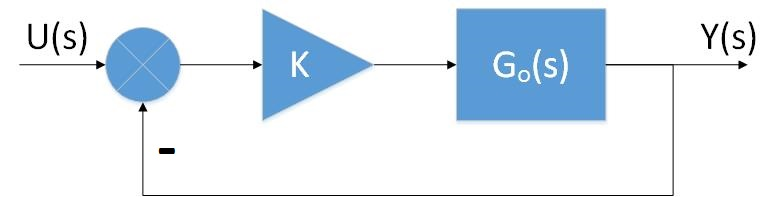
\includegraphics[width=4in]{servo.jpg}
	\captionsource{Schemat blokowy serwomechanizmu.}{Własne}
\end{figure}

\(G_o(s)\) jest transmitancją silnika prądu stałego, gdy wejściem jest napięcie, a położenie kątowe wału silnika:
\begin{equation}
G_o(s)=\frac{1}{s(Ts+1)}
\end{equation}
\(K\) jest wzmocnieniem regulatora proporcjonalnego.\newline
Transmitancja zastępcza powyższego układu wynosi:
\begin{equation}
\label{eq:servo}
G_s(s)=\frac{K}{Ts^2+s+K}
\end{equation}
Ze względu na brak enkoderów w układzie, nie można przeprowadzić identyfikacji parametrów serwomechanizmów. Na podstawie obserwacji wiadomo, że w wzmocnienie regulatora jest dobrane tak, by silnik nie oscylował wokół wartości zadanej. Powinno być ono wzmocnieniem krytycznym dla danego silnika. Aby wzmocnienie \(K\) było krytyczne, musi być ono równe:
\begin{equation}
\label{eq:kryt}
K=\frac{1}{4T}
\end{equation}
Podstawiając powyższy wzór do równania \ref{eq:servo} otrzymuje się:
\begin{equation}
G_s(s)=\frac{1}{4T^2s^2+4Ts+1}
\end{equation}
Wartość stałej czasowej jest przyjęta na podstawie odpowiedzi skokowej serwomechanizmu.
\begin{equation}
T=0.05
\end{equation}
Następnie wykonano schemat blokowy kompletnego układu (z kamerą i implementowanym regulatorem).

\begin{figure}[h]
	\centering
	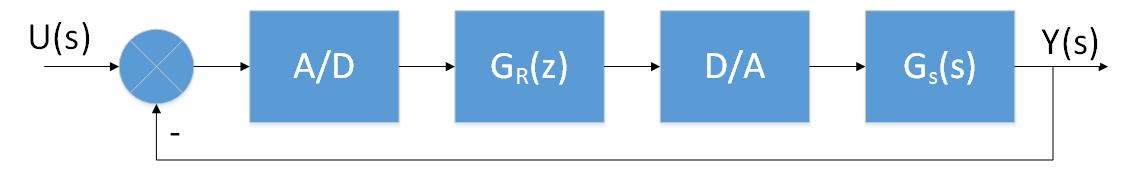
\includegraphics[width=4in]{uklad.jpg}
	\captionsource{Schemat blokowy kompletnego układu.}{Własne}
\end{figure}

\(G_R(z)\) jest transmitancją projektowanego regulatora dyskretnego.
\paragraph*{}
Rolę przetwornika A/D pełni w układzie kamera, a przetwornika D/A sterownik serwomechanizmów. Schemat ten można przedstawić w następującej, równoważnej postaci.

\begin{figure}[h]
	\centering
	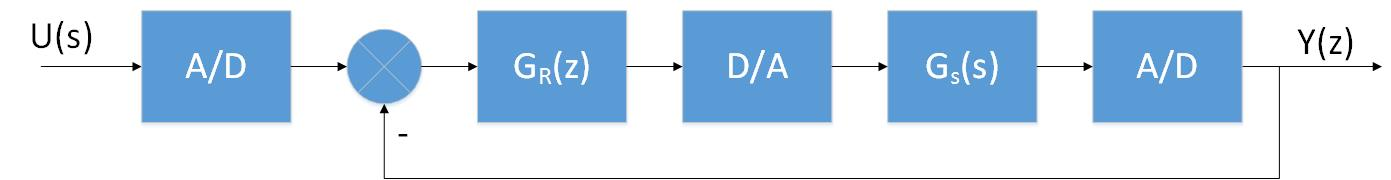
\includegraphics[width=4in]{uklad_digital.jpg}
	\captionsource{Równoważny schemat kompletnego układu.}{Własne}
\end{figure}

Transmitancję opisaną równaniem \ref{eq:servo} można zapisać za pomocą równań stanu:
\begin{equation}
\dot{x}=Ax+Bu
\end{equation}
\begin{equation}
y=Cx
\end{equation}
\begin{equation}
A=
	\begin{bmatrix}
	0 & 1 \\
	-\frac{K}{T} & -\frac{1}{T}
	\end{bmatrix}
\end{equation}
\begin{equation}
B=
	\begin{bmatrix}
	0 \\
	1
	\end{bmatrix}
\end{equation}
\begin{equation}
C=
	\begin{bmatrix}
	\frac{K}{T} & 0
	\end{bmatrix}
\end{equation}
Wzmocnienie krytyczne regulatora w serwomechanizmach dobrane jest dla silników bez obciążenia. Jeśli silnik zostaje obciążony, to zwiększa się jego stała czasowa. Wzmocnienie więc również powinno być zmienione. Wziąć należy jednak pod uwagę, że masa użytej kamery jest mała w porównaniu do maksymalnej masy obciążenia tych urządzeń. Z tego względu można przyjąć, że stała czasowa nie zmienia się, a wzmocnienie nadal jest krytyczne. Nadal zachodzi więc równanie \ref{eq:kryt}. Podstawiono je do powyższych macierzy.
\begin{equation}
A=
	\begin{bmatrix}
	0 & 1 \\
	-\frac{1}{4T^2} & -\frac{1}{T}
	\end{bmatrix}
\end{equation}
\begin{equation}
B=
	\begin{bmatrix}
	0 \\
	1
	\end{bmatrix}
\end{equation}
\begin{equation}
C=
	\begin{bmatrix}
	\frac{1}{4T^2} & 0
	\end{bmatrix}
\end{equation}
Obiekt ten można razem z przetwornikiem A/D i przetwornikiem D/A pierwszego rzędu przedstawić można jako jeden równoważny obiekt dyskretny. Wyznaczono następnie równania stanu tego obiektu \cite{TS}.
\begin{equation}
\label{eq:A^+}
A^+=e^{hA}
\end{equation}
\begin{equation}
\label{eq:B^+}
B^+=\int\limits_{0}^{h}e^{tA}Bdt
\end{equation}
\begin{equation}
C^+=C
\end{equation}
\(h\) oznacza okres próbkowania dyskretnej części układu.
\begin{equation}
h=\frac{1}{60}
\end{equation}
Obliczenia rozpoczęto od wyliczenia macierzy \(e^{tA}\).
\begin{equation}
e^{tA}=\mathcal{L}^{-1}[(sI-A)^{-1}]
\end{equation}
\begin{equation}
e^{tA}=\mathcal{L}^{-1}
	\begin{bmatrix}
	\frac{s+\frac{1}{T}}{(s+\frac{1}{2T})^2} & \frac{1}{(s+\frac{1}{2T})^2} \\
	\frac{-\frac{1}{4T^2}}{(s+\frac{1}{2T})^2} &  \frac{s}{(s+\frac{1}{2T})^2}
	\end{bmatrix}
\end{equation}
\begin{equation}
\label{eq:e^tA}
e^{tA}=
	\begin{bmatrix}
	(1+\frac{t}{2T})e^{-\frac{t}{2T}} & te^{-\frac{t}{2T}} \\
	-\frac{t}{4T^2}e^{-\frac{t}{2T}} & (1-\frac{t}{2T})e^{-\frac{t}{2T}}
	\end{bmatrix}
\end{equation}
Podstawiono \ref{eq:e^tA} do \ref{eq:A^+} i \ref{eq:B^+}.
\begin{equation}
A^+=
	\begin{bmatrix}
	(1+\frac{h}{2T})e^{-\frac{h}{2T}} & he^{-\frac{h}{2T}} \\
	-\frac{h}{4T^2}e^{-\frac{h}{2T}} & (1-\frac{h}{2T})e^{-\frac{h}{2T}}
	\end{bmatrix}
\end{equation}
\begin{equation}
B^+=\int\limits_{0}^{h}
	\begin{bmatrix}
	te^{-\frac{t}{2T}} \\
	(1-\frac{t}{2T})e^{-\frac{t}{2T}}
	\end{bmatrix}
	dt
\end{equation}
\begin{equation}
\int te^{-\frac{t}{2T}}=-2Tte^{-\frac{t}{2T}}+2T\int e^{-\frac{t}{2T}}dt
\end{equation}
\begin{equation}
\int te^{-\frac{t}{2T}}=-2Tte^{-\frac{t}{2T}}-4T^2e^{-\frac{t}{2T}}
\end{equation}
\begin{equation}
B^+=
	\begin{bmatrix}
	-2T(h+2T)e^{-\frac{h}{2T}}+4T^2 \\
	he^{-\frac{h}{2T}}
	\end{bmatrix}
\end{equation}
\begin{equation}
C^+=
	\begin{bmatrix}
	\frac{1}{4T^2} & 0
	\end{bmatrix}
\end{equation}
Aby sprawdzić poprawność przeprowadzonych obliczeń postanowiono porównać odpowiedzi skokowe układu ciągłego i dyskretnego. Do tego celu zostało wykorzystane środowisko \textit{MATLAB}.

\begin{figure}[h]
	\centering
	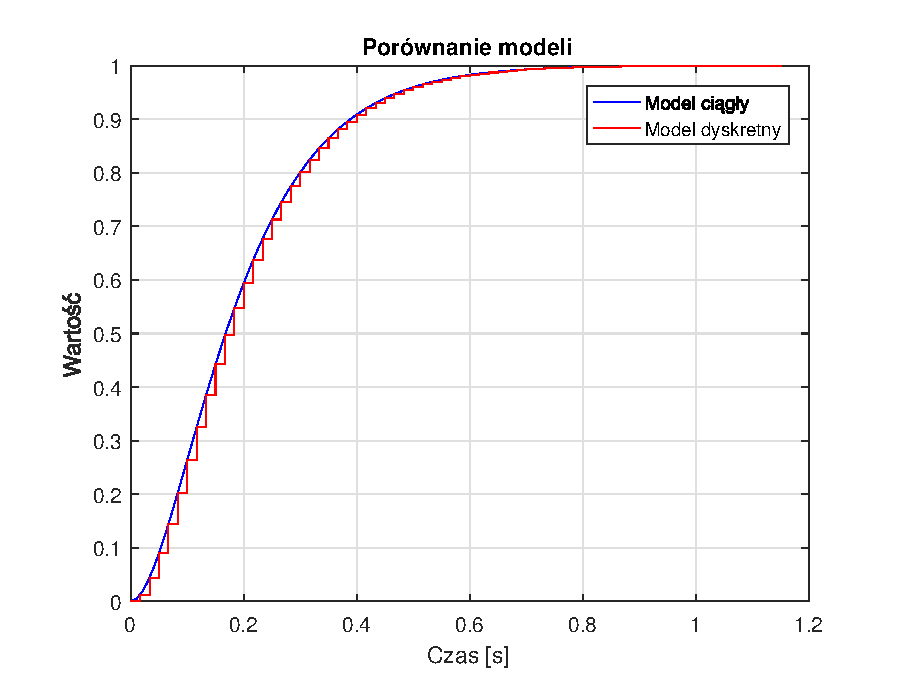
\includegraphics[width=4in]{comp.eps}
	\captionsource{Porównanie modelu ciągłego oraz odpowiadającego mu dyskretnego.}{Własne}
\end{figure}

Na podstawie powyższego wykresu można wnioskować, że wyliczony model jest poprawny. Należy jednak zwrócić uwagę na fakt, że w rzeczywistym układzie występują występują dodatkowo opóźnienia, które nie zostały uwzględnione w modelu. Z tego względu model nie będzie idealnie odpowiadał działaniu rzeczywistego układu.

\paragraph*{}
Kompletny model układu postanowiono zaimplementować w programie \textit{Simulink}. Uwzględnia on:
\begin{itemize}
\item Nasycenie wartości zadanej serwomechanizmów
\item Przeliczanie współrzędnych śledzonego obiektu na kąty
\item Obliczanie szerokości impulsów wysyłanych do serwomechanizmu
\item Kwantyzację liczby pikseli i szerokości impulsów
\end{itemize}

\begin{figure}[h]
	\centering
	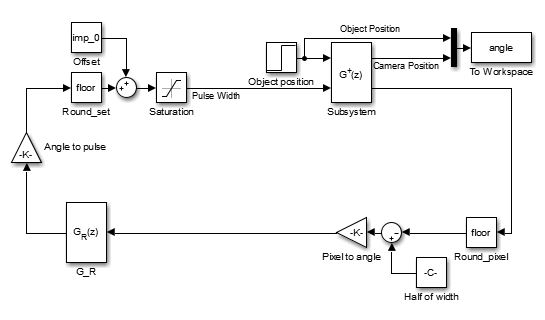
\includegraphics[width=4in]{Simulink.jpg}
	\captionsource{Model układu zrealizowany w programie \textit{Simulink}.}{Własne}
\end{figure}

\section{Projekt regulatora}
\label{sec:projektregulatora}

W układzie nie ma czujnika pozycji serwomechanizmów, więc algorytm regulacji musi bazować na wyjściu z poprzedniej iteracji. Algorytmem, który działa w ten sposób jest prędkościowy (przyrostowy) regulator PID. Zaimplementowany regulator ma następującą postać:
\begin{equation}
u(k)-u(k-1)=P \cdot (e(k)-e(k-1))+I \cdot e(k)+D \cdot (e(k)-2e(k-1)+e(k-2))
\end{equation}
Został on zrealizowany w programie \textit{Simulink}.

\begin{figure}[h]
	\centering
	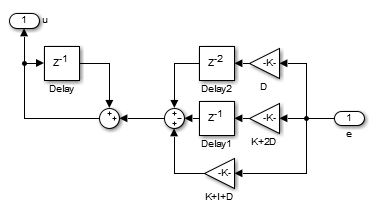
\includegraphics[width=4in]{Przyrostowy.jpg}
	\captionsource{Realizacja przyrostowego regulatora PID.}{Własne}
\end{figure}

Na podstawie odpowiedzi modelu dobrano następujące wartości parametrów:
\begin{equation}
P=1
\end{equation}
\begin{equation}
I=0.1
\end{equation}
\begin{equation}
D=0.2
\end{equation}

\begin{figure}[H]
	\centering
	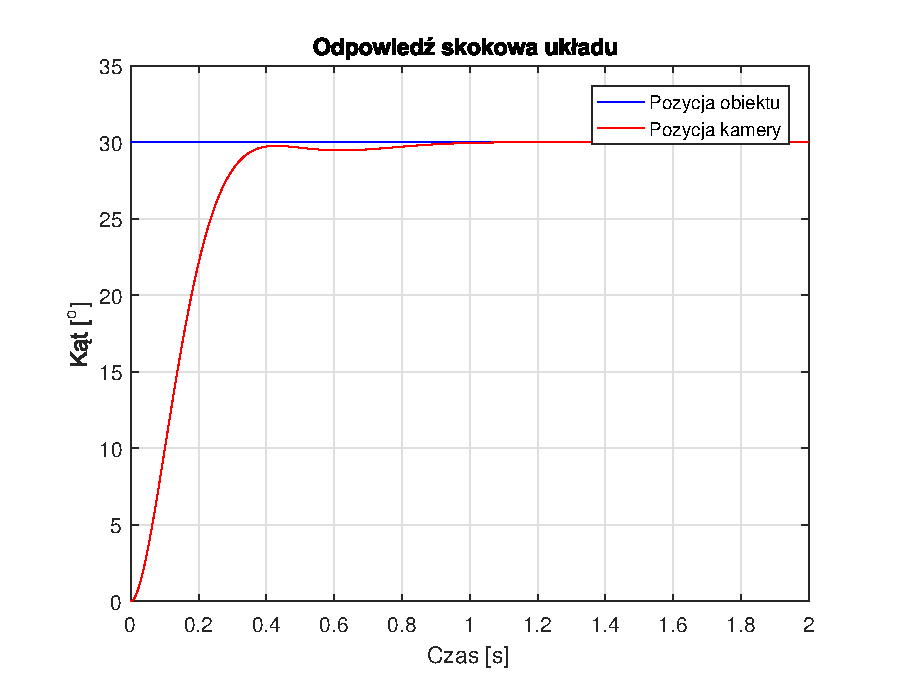
\includegraphics[width=3.4in]{sim_step.eps}
	\captionsource{Odpowiedź skokowa układu z dobranym regulatorem.}{Własne}
\label{fig:sim_step}
\end{figure}

\begin{figure}[H]
	\centering
	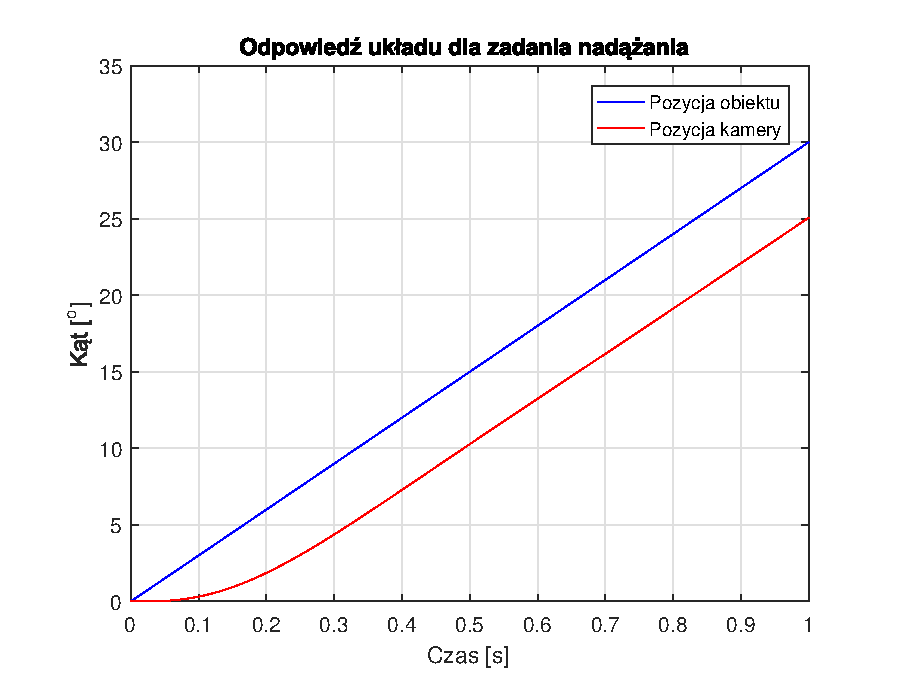
\includegraphics[width=3.4in]{sim_ramp.eps}
	\captionsource{Odpowiedź układu dla zadania nadążania.}{Własne}
\label{fig:sim_ramp}
\end{figure}

Na wykresie \ref{fig:sim_step} widać, że układ szybko reaguje na skokowe zmiany pozycji śledzonego obiektu. Z kolei na wykresie \ref{fig:sim_ramp} zauważyć można, że obecny jest uchyb ustalony dla zadania nadążania. Aby się go pozbyć konieczne byłoby zastosowanie w układzie dodatkowego członu całkującego szeregowo użytym regulatorze, co zwiększyłoby rząd stosowanego rozwiązania. Użyte parametry mogą zostać skorygowane w rzeczywistym układzie w zależności od rezultatów i wpływu pominiętych efektów.